\RequirePackage{mathtools}
\documentclass{llncs}
\pagestyle{plain}
%%%%%%%%%%%%%%%%%%%% Graphicx %%%%%%%%%%%%%%%%%%%%%%%%%%%%%%%%%%%%
\usepackage{graphicx}
\usepackage{xcolor}
\usepackage[caption=false]{subfig}
%%%%%%%%%%%%%%%%%%%%%%%%%%%%%%%%%%%%%%%%%%%%%%%%%%%%%%%%%%%%%%%%%%

%%%%%%%%%%%%%%%%%%%% ALGORITHMIC STUFF %%%%%%%%%%%%%%%%%%%%%%%%%%%
\usepackage{algorithm}
\usepackage{algorithmicx}
\usepackage{algpseudocode}
\newcommand*\Let[2]{\State #1 $\gets$ #2}
\newtheorem{assumption}{Assumption}
%%%%%%%%%%%%%%%%%%%%%%%%%%%%%%%%%%%%%%%%%%%%%%%%%%%%%%%%%%%%%%%%%%

%%%%%%%%%%%%%%%%%%%% THEOREM STUFF %%%%%%%%%%%%%%%%%%%%%%%%%%%%%%%
\usepackage{mathtools}
\usepackage{amssymb}
\usepackage{amsmath}
\usepackage{url}
%%%%%%%%%%%%%%%%%%%%%%%%%%%%%%%%%%%%%%%%%%%%%%%%%%%%%%%%%%%%%%%%%%
\graphicspath{{../pics/}{../pics/new_fig/}}

%\usepackage{ulem}
%\newcommand\add[1]{\textcolor{olive}{#1}} 
%\newcommand\del[1]{\textcolor{red}{#1}} 
\newcommand\del[1]{} 
\newcommand\add[1]{#1} 
%\newcommand\rep[2]{\textcolor{red}{\sout{#1}}\textcolor{olive}{#2}}

\usepackage{todonotes}
\usepackage{soul}
%\newcommand{\hlfix}[2]{\todo{#2}{\texthl{#1}}}
%\newcommand{\aldid}[2]{\todo[backgroundcolor=blue!20]{AL : #2}{\texthl{#1}}}
%\newcommand{\gdadid}[2]{\todo[backgroundcolor=blue!41]{GDA : #2}{\texthl{#1}}}

\title{On the Bright Side of Darkness: \\
Side-Channel Based Authentication Protocol Against Relay Attacks}
\author{Anonymous submission to WISTP 2018}
\institute{}

\begin{document}
\maketitle

\begin{abstract}
Relay attacks are nowadays well known and most designers of secure authentication protocols are aware of them. At present, the main methods to prevent these attacks are based on the so-called distance bounding technique which consists in measuring the round-trip time of the exchanged authentication messages between the prover and the verifier to estimate an upper
bound on the distance between these entities. 
Based on this bound, the verifier checks if the prover is sufficiently close by to rule out an unauthorized entity.
Recently, a new work has proposed an authentication protocol that surprisingly uses the side-channel leakage to prevent relay attacks. 
In this paper, we exhibit some practical and security issues of this protocol and provide a new one that fixes all of them. 
Then, we argue the resistance of our proposal against both side-channel and relay attacks under some realistic assumptions. 
Our experimental results show the efficiency of our protocol in terms of false acceptance and false rejection rates.

\end{abstract}
{\bf Keywords:} authentication protocol, relay attacks, side-channel attacks, physical leakage. 

\section{Introduction}
\subsubsection{Relay Attacks VS Authentication Protocols.}
A \textit{relay attack} is a form of \textit{man-in-the-middle} attack where the attacker merely relays the verbatim messages between a verifier and a prover, to authenticate to the verifier as a legitimate prover. In such a context, the attacker is usually close to the verifier and claims being the legitimate prover while the latter is not in the neighborhood. Such an attack is particularly well-suited to get around access controls, \emph{e.g.} to get inside a secure location or to unlock the doors of a vehicle.
Without loss of generality, we shall consider in the sequel that the prover is a contactless Secure Element (SE) and the verifier is a contactless reader. 

The current trend to include Near Field Communication (NFC) (ISO/IEC $14443$) technology into mobile phones significantly simplifies skimming and relay attacks. Although the NFC protocol requires that the prover and the verifier are in close proximity, this constraint does not help to counteract relay attacks. Indeed, in \cite{Hancke05apractical} it is shown how to set up a relay attack by placing a {\em proxy-token} in the range of a contactless reader to relay queries from the verifier to a {\em mole} which forwards to the genuine prover the requests from the genuine verifier. The mole also sends back the responses from the genuine prover to the proxy-token which delivers them to the genuine verifier. Most recently the authors in \cite{DBLP:journals/iacr/FrancisHMM11,MendozaNFC} have shown how smartphones equipped with an NFC antenna can be used efficiently as a generic relay attack platform.

To thwart relay attacks, Brands and Chaum introduced in $1993$ the so-called \textit{distance bounding protocols}~\cite{Brands1994}.

The core idea of these protocols is to measure the round-trip time of the authentication messages exchanged between the prover and the verifier. Then, based on this propagation time, the verifier decides whether the prover is within the distance and hence discriminates a legitimate prover from an attacker.
Although the idea has been introduced many years ago, it is only quite recently that distance bounding protocols have been investigated and several designs have been 
proposed in the literature~\cite{DBLP:conf/fps/BrelurutGL15,DBLP:conf/wisec/TippenhauerLKC15}.

\subsubsection{On the Bright Side of Side-Channel Leakage.}
Before detailing our proposal, we provide in this section a survey of some recent research lines suggesting the use of side-channel information constructively to enhance, or as an alternative to, existing cryptographic protocols.
	
To avoid counterfeiting of Integrated Circuits (ICs), authors in \cite{DBLP:conf/socc/MarchandBJ14} have proposed a watermarking based technique. It consists in inserting a software manipulating a sensitive variable which simply computes the Exclusive-OR (XOR) operation between an internal $8$-bit counter and an $8$-bit secret key and then applies the Sbox of the AES to the result of the XOR. The internal counter increases its value on each run of the software. 
To check whether a device is genuine or not, the issuer of the device provides a reference device containing the same software as in the device under test (if the latter is not a counterfeit). By measuring several power traces from both devices and then by computing the degree of correlation between their respective leakages, the issuer can conclude that the audited device is a legal copy if the correlation is sufficiently high (\emph{i.e.} greater than a fixed threshold). 
Unfortunately, the authors only use an $8$-bit length key. Moreover, each time it is required to check the authenticity of a device, the internal $8$-bit counter is reset on both devices (the device under test as well as the reference device), making the sequence predictable and subject to side-channel attacks\footnote{If the reset value of the internal counter is unknown to the attacker, she must recover it, which is far from being an issue since it is only an $8$-bit value.}. 

In another work, Kerckhof \emph{et al.} in \cite{DBLP:conf/host/KerckhofDSG13} have used some techniques from side-channel analysis still in the context of IP protection. 
The typical use case on which they have focused on is the implementation of some customized ciphering algorithms. 
An estimation of the coefficient of correlation is again used but now (despite of the context of symmetric ciphers), no sensitive variable is involved in the computation of the correlation. 
The authors have rather used the correlation as a tool to correlate features extracted from an acquired signal (which represents the execution of a specific implementation without paying attention to the manipulated data) with features extracted from a reference device embedding the same IP as in the device under test. 
Several other works have suggested to use side channel for IC fingerprinting or Trojan detection~\cite{7256167,10.1007/978-3-642-15031-9_12}. \del{In most of the cases, it is required to have a reference design to exploit the leakage.}


To avoid relay attacks, authors in~\cite{SakiyamaMMKHMMN15} and \cite{DBLP:conf/ccs/ReidNTS07} have proposed authentication protocols based on the use of physical leakage.
In \cite{DBLP:conf/ccs/ReidNTS07}, the authors simply suggested the use of a dedicated binary xor instruction which, depending on the resulting bit, leaks exaggeratedly (\emph{e.g.} if the resulting bit is $1$) or not (\emph{e.g.} if the resulting bit is $0$). Such a technique allows the authors to only use a so-called simple side-channel analysis.
In \cite{SakiyamaMMKHMMN15}, the prover performs on his side some cryptographic computations while the verifier acquires the corresponding physical leakage (\emph{e.g.} the electromagnetic radiation).
Assuming that the verifier and the prover share a symmetric key $K$, the verifier analyses the leakage generated by a nearby SE and authenticates it ``physically'' if the correlation between the acquired leakage and the associated predictions made by the verifier is sufficiently high. Such an authentication associating classical authentication techniques with statistical side-channel analysis is called \textit{side-channel authentication}.  
\add{According to us, this new paradigm is really interesting since it may indeed allow to detect relay attacks in the field. The fact that it is required to acquire the electro-magnetic signal of the prover (which is is typically a smartcard) may not be unrealistic depending on the considered use case. We acknowledge that adding the means for signal acquisition in a so-called  payment terminal is probably not an option. This situation is not so clear when talking about relay attacks on car immobilizers (where the key is more or less a smartcard) or when talking about control access to a public transport network. In both cases it would surely be possible to embed an equipment to acquire the leakage of the prover: inside the driver's door of the car and inside the entrance gate to the public transport network. Of course this countermeasure comes at a price and its implementation will depend on how relay attacks impact the overall fraud.}
%This is because the leakage of the SE can be acquired by the verifier if the SE is physically nearby the verifier.

\subsubsection{Our Contribution.}
In this work, we propose a new authentication protocol that $(1)$ follows the side-channel based approach suggested in \cite{SakiyamaMMKHMMN15} and \cite{DBLP:conf/ccs/ReidNTS07} and $(2)$ fixes its practical and security issues that we detail hereafter.
According to our understanding, in \cite{SakiyamaMMKHMMN15} the authors propose four schemes in which both parties, the prover and the verifier, share a symmetric key $K$ that is used to perform AES computations (on both sides) using this secret key. The inputs of the AES computations are specified differently depending on the design that is considered. The main drawback of their proposal is that a customized $N$-round AES is required ($N=1.000$ rounds in their experiments). 

From a design point of view, this design constraint raises an issue because in the context of secure element only standardized cryptographic primitives should be considered (\emph{i.e.} AES-$128$, AES-$192$ and AES-$256$). 
From a security perspective, the protocol proposed in \cite{SakiyamaMMKHMMN15} has some flaws that could be exploited by performing some side-channel attacks. The proposed $N$-round AES implementations are not protected against side-channel attacks. So, an adversary who can recover the physical leakage, is able to perform a statistical attack to recover the shared master key $K$.
The reason behind not using the well-known side-channel countermeasures (\emph{e.g.} masking, secret sharing) is that the leaked information is no longer exploitable and so the physical authentication cannot succeed.  

Finally, from a practical perspective, assuming that the leakage model is uniform over the whole intermediate values of the $N$-round customized AES~\cite{SakiyamaMMKHMMN15} is unsound in real hardware due to small load imbalances, process variations, routing, \emph{etc}. For instance, authors in~\cite{10.1007/978-3-642-42033-7_26} have characterized using a stochastic approach the leakage of four successive AES Sbox outputs.
The obtained results prove that the leakage is very unbalanced for each Sbox. Hence, in practice the authentication may fail since the correlation between the acquired leakage and the associated predictions may be too low when following such assumption on the leakage model.

To overcome these issues and to resist relay attacks, we propose a new authentication protocol that first ensures that only a genuine verifier can exploit the leakage from a prover, \emph{i.e.} no attacker should be able to mount an attack based on side-channel analysis to recover the secret key $K$. Second, this protocol only uses standard cryptographic primitives (\emph{i.e.} AES-$128$, AES-$192$ or AES-$256$).

Throughout several practical experiments (see Sec.~\ref{sec:simu}), we argue that our proposal is secure against both side-channel attacks and relay attacks under some realistic assumptions.

\subsubsection{Paper Outline.}
The paper is organized as follows. In Sec.~\ref{sec:background}, we briefly describe the AES block cipher and provide some useful notations. Then, in Sec.~\ref{sec:protocol} we describe our new authentication protocol. To assess the efficiency of our proposal, a practical security evaluation is conducted in Sec.~\ref{sec:simu}. Finally, Sec.~\ref{sec:conc} draws general conclusions and opens some perspectives for future work.

\section{Background}\label{sec:background}

%!TEX root = physical_authent.tex
\subsection{AES}~\label{ssec:AES}
The Advanced Encryption Standard (AES)~\cite{FIPS197} is a \del{symmetric} block cipher that processes data blocks of $128$ bits length and a variable secret key length ($128$, $192$ or $256$ bits). Hence, as specified by the standard~\cite{FIPS197}, three different block-ciphers can be used: AES-$128$, AES-$192$, AES-$256$.
Depending on the length of the key, the AES performs $N_r$ rounds, with $N_r \in [10, 12, 14 ]$. The AES manipulates, all along its execution, an internal state which is a $(4 \times 4) $ matrix of bytes.

\begin{algorithm}[ht!]
	\caption{The Advanced Encryption Standard (AES)}\label{alg:AES}
	\begin{algorithmic}[1]
	\Require{$In$: the $128$-bit input, $N_r$: the number of rounds, $(k_i)_{0 \leq i \leq  N_r}$: the round keys}
	\Ensure{$Out$: the $128$-bit output}
	\State $M_{-1} = In$	
	\For{$i = 0 \textbf{ to } N_r-2$}
		\State $X_i = \mbox{AddRoundKey}(M_{i-1},k_{i})$
		\State $Y_i = \mbox{SubBytes}(X_{i})$
		\State $S_i = \mbox{ShiftRows}(Y_{i})$
		\State $M_i = \mbox{MixColumns}(S_i)$
    \EndFor
    \State $X_{N_r-1} = \mbox{AddRoundKey}(M_{N_r-2}, k_{N_r-1})$
   	\State $Y_{N_r-1} = \mbox{SubBytes}(X_{N_r-1})$
	\State $S_{N_r-1} = \mbox{ShiftRows}(Y_{N_r-1})$
	\State $Out = X_{N_r} = \mbox{AddRoundKey}(S_{N_r-1}, k_{N_r})$
	\State \Return $Out$
  	\end{algorithmic}
\end{algorithm}

The AES involves four main operations: AddRoundKey, SubBytes, ShiftRows and MixColumns. As shown in Algorithm~\ref{alg:AES}, at the $i^{\text{th}}$ round these operations yield the so-called intermediate states of the AES and are denoted resp. by $X_i$, $Y_i$, $S_i$ and $M_i$. A byte from an intermediate state, say $X_i$, is denoted by ${X_i[l,c]}$ with $(l,c) \in {[0,3]}^2$ in the sequel.


\subsection{Leakage Model}\label{ssec:leak}
Let $V$ be a sensitive byte (\emph{e.g.} the variable $Y_i[l,c]$ of the $i^{\text{th}}$ AES round), then it is often assumed that the leakage function $L(V)$ is well modeled by:
\begin{equation}
L(V) = \alpha_t \cdot \mbox{HW}(V) + \beta_t + W \enspace , \text{where:}
\label{eq:leak}
\end{equation}

\begin{enumerate}
\item $ \text{HW}(.)$ is the Hamming Weight function.
\item $W$ is a Gaussian noise $\mathcal{N}(0,\sigma)$ with null mean and standard deviation $\sigma$.
\item $(\alpha_t, \beta_t)$ are some weighting values specific to each targeted sensitive byte of index $(l,c)$ of the $i^{\text{th}}$ AES round (\emph{i.e.} $t = (l,c,i)$).
\end{enumerate}  

\add{It is worthy to note that, in some specific cases, the real leakage function can be slightly different from the model we considered in~\eqref{eq:leak}. In such a case, one have to characterize the real leakage function by applying a \textit{stochastic approach} as suggested in~\cite{10.1007/11545262_3}. For the sake of simplicity, we assume that leakage function follows the model described in~\eqref{eq:leak}. In the meantime, we stress the fact that our proposal works well with any leakage function.}


\section{Protocol Proposal}\label{sec:protocol}
%!TEX root = physical_authent.tex
As mentioned in the introduction, the protocol must ensure that only a genuine verifier can exploit the leakage from a prover, while avoiding any attacker attempting to mount a side-channel analysis. It must also consider some practical constraints such as the use of standard cryptographic APIs (\emph{i.e.} avoiding customized AES implementations as required in \cite{SakiyamaMMKHMMN15} for instance). 

\subsection{Adversarial Model}
In the sequel, we shall consider the following assumptions.
\begin{assumption}[\textbf{Attacker's profile}]
\label{assump_1}
We consider an attacker who can perform $(1)$ side-channel attacks by capturing the side-channel leakage of the prover to try retrieving the secret key and $(2)$ relay attacks to try authenticating to a verifier as a genuine prover. 
\end{assumption}


\begin{assumption}[\textbf{Impracticability of reproducing the physical leakage}]
\label{assump_2}
We assume that it is significantly difficult in practice for an attacker performing a relay attack to generate a copy of the side-channel information leaked by the genuine prover. This assumption is quite realistic and is merely justified in Sec.~\ref{ssec:security}.
\end{assumption}


Assumption~\ref{assump_2} relies on the fact that even if an attacker succeeds in capturing, copying and replaying the side-channel leakage, then this procedure will take some time denoted $\Delta$. Thus, replaying the side-channel information is equivalent to add some desynchronization in the trace which is well known to reduce the degree of correlation~\cite{DBLP:books/daglib/0017272}.


\subsection{Protocol Specification}
\label{sec_proposal}
\subsubsection{Overall Description.}\label{sssec:overall}
We provide in Fig.~\ref{fig:protocol} an overview of our protocol. 
First, we assume that the master key $K$ has already been shared between the verifier and the prover (\emph{e.g.} either loaded during the personalization phase of the prover or by using the classical Diffie-Hellman key exchange protocol with certified public keys on both sides).
\add{The prover initiates the protocol by sending $R_P$ (a $128$-bit random value) to the verifier who replies by sending $R_V$ (a $128$-bit random value). Both then use $R_V\oplus R_P$ (as an alternative one could use $R_V||R_P$)} as an input to a secure \textit{Key Derivation Function}, denoted KDF in Fig.~\ref{fig:protocol}, to generate $2N$ session keys $(K_0^{(0)}, K_1^{(0)}, \cdots, K_{2N-1}^{(0)}) = (K_0, K_1, \cdots, K_{2N-1})$ using the shared master key $K$.
This secure KDF (\emph{i.e.} orange box in Fig.~\ref{fig:protocol}) must be protected against classical side-channel attacks by implementing for instance some well-known masking countermeasures (see \emph{e.g.}~\cite{DBLP:conf/eurocrypt/Coron14,DBLP:conf/ches/GenellePQ11,DBLP:conf/ches/RivainP10}). In addition, the verifier generates $q \times 2N$ extra random keys denoted $(K_0^{(i)}, K_1^{(i)}, \dots, K_{2N-1}^{(i)})$ for $i \in [1,q]$. Now, to fix the practical issues of the protocol proposed in \cite{SakiyamaMMKHMMN15}, we use a set of $N$ AES encryption (\emph{i.e.} the 	blue boxes in Fig.~\ref{fig:protocol}) instead of a customized $N$-round AES. 
These AES executions, denoted \textit{leaky AES} in the sequel, do not implement any countermeasure against side-channel analysis and are used to encipher the last $N$ session keys

$(K_N, \cdots, K_{2N-1})$ using the first $N$ ones $(K_0, K_1, \cdots, K_{N-1})$ as encryption keys.\newline
On the prover side, the $i^{\text{th}}$ AES encryption provides $C_i = \mbox{AES}_{K_i}(K_{i+N})$ and leaks all intermediate sensitive variables which are measured by the verifier.

The verifier on its side, computes $q+1$ such sequences of $N$ AES and stores all relevant intermediate sensitive variables. The $j^\text{th}$ output of the $i^\text{th}$ sequence of $N$ AES is denoted $C_j^{(i)} = \mbox{AES}_{K_j^{(i)}}(K_{j+N}^{(i)})$ for $j$ in $[0,N-1]$ and $i$ in $[0,q]$.
Then, for each $i^\text{th}$ executed sequence of $N$ AES, the verifier computes a likelihood value $\mathcal{L}_i$ between the corresponding stored intermediate values and the acquired measurement while the prover was executing its $N$ leaky AES.

At the end of this step, the verifier holds $q+1$ likelihood values $\mathcal{L}_i$ with $i$ in $[0, q]$.
If the prover is genuine, then the maximum value of likelihood should be $\mathcal{L}_0$ (since obtained using the  session keys derived from the shared master key $K$) and a gap should exist between $\mathcal{L}_0$ and $\{\mathcal{L}_{i}\}_{i\in [1,q]}$ (denoted $\{\mathcal{L}_{i\not=0}\}$ in the sequel).
If the greatest likelihood value is not $\mathcal{L}_0$ or if $\mathcal{L}_0$ does not stand out from $\{\mathcal{L}_{i\not=0}\}$, then the authentication is rejected and the protocol ends.
Otherwise, the verifier continues the protocol by sending the ciphertext $C_k^{(0)}$ where $k$ is chosen randomly in $[0, N-1]$.

Upon receiving $C_k^{(0)}$, the prover checks whether it belongs to the set of ciphertexts it has computed (\emph{i.e.} whether it exists $l$ in $[0, N-1]$ \emph{s.t.} $C_l = C_k^{(0)}$) and if so, sends back a different ciphertext $C_m$ (\emph{i.e.} $ m \neq l$). Otherwise, the prover rejects the authentication. The verifier finally checks whether it holds $C_l^{(0)}$ such that $C_l^{(0)} = C_m$. If it is the case the verifier and the prover are mutually and physically authenticated.

\begin{figure}[ht!]
   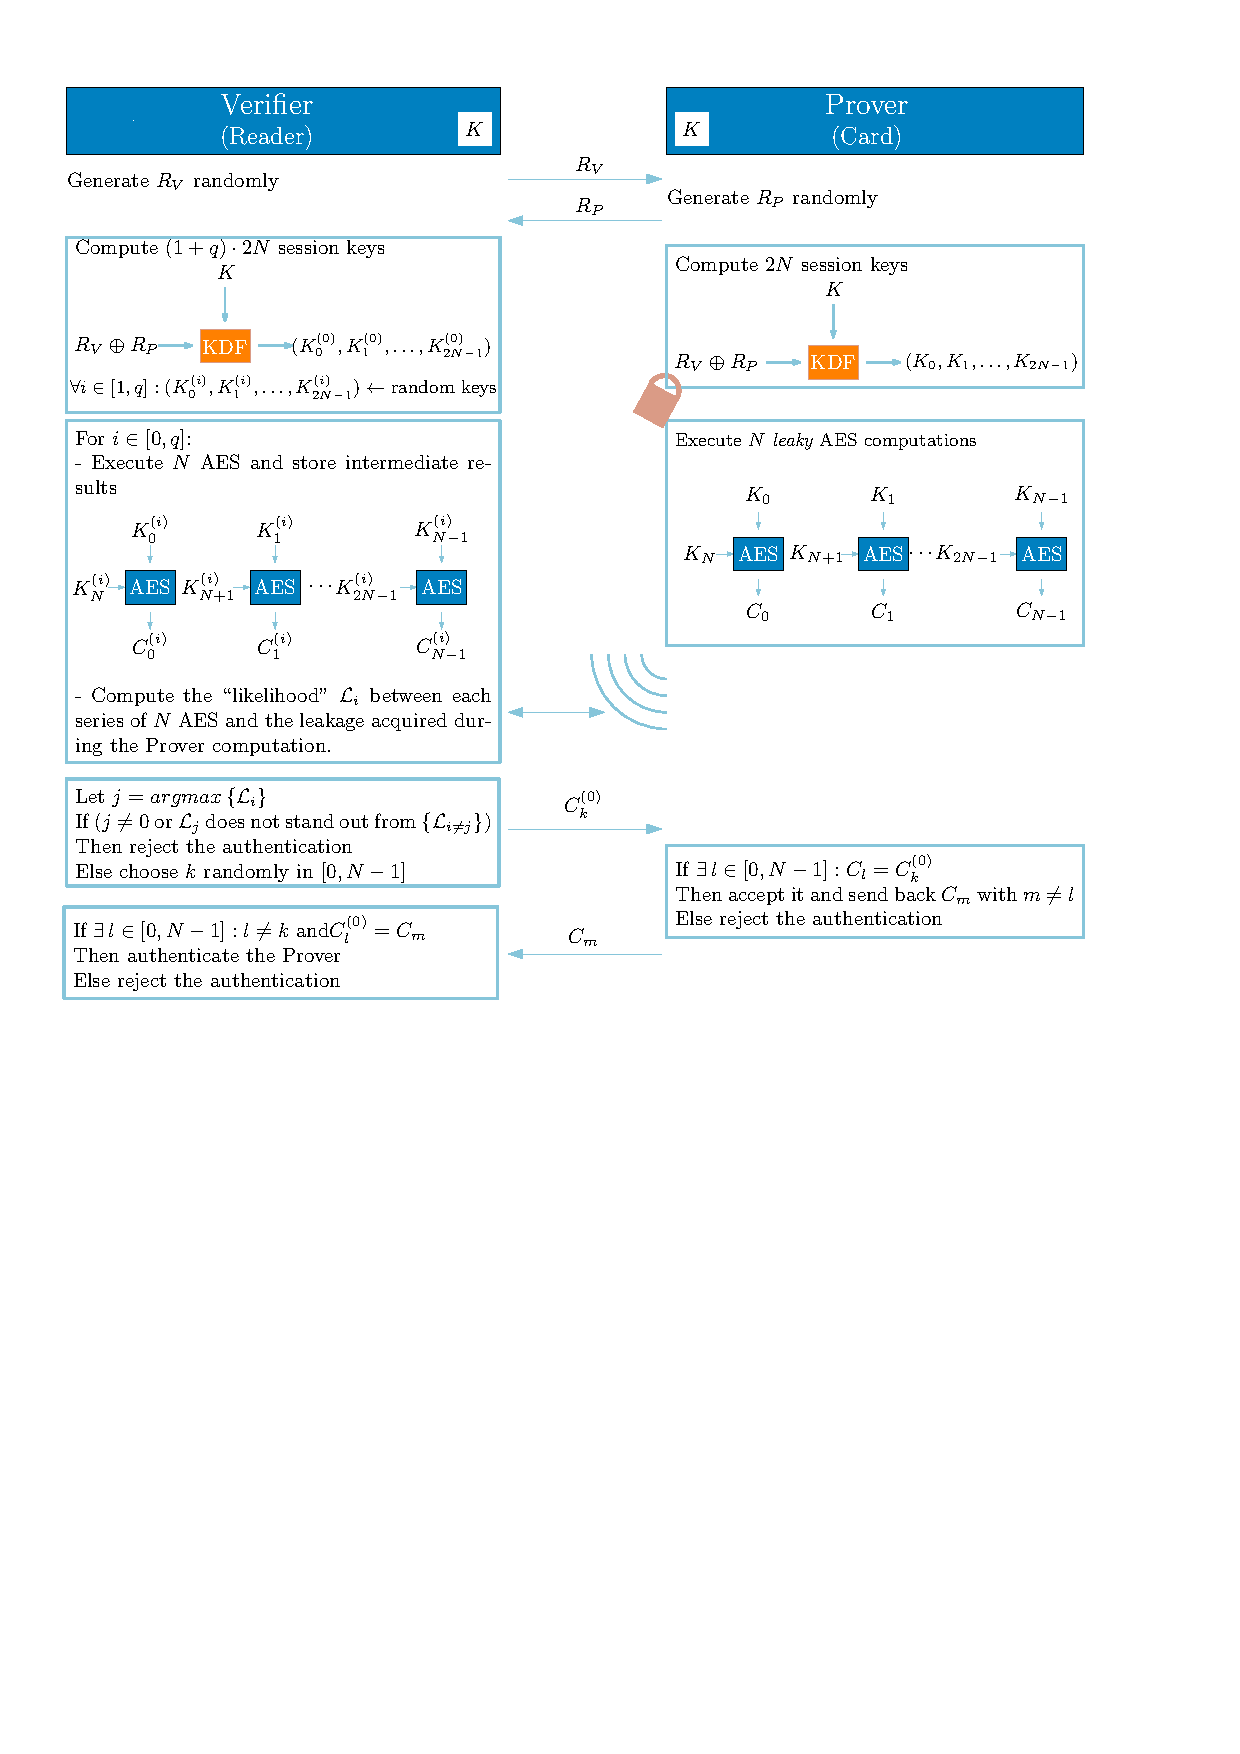
\includegraphics[width=1.0\linewidth]{../pics/protocol_2N-1.pdf}
   \caption{Description of the physical authentication protocol.} \label{fig:protocol}
\end{figure}

The most critical step for the success of our protocol is the acquisition of the physical leakage since it requires a perfect synchronization between the prover and the verifier.
To ensure this, a trick would consist in triggering a timer, at the verifier side, upon sending the random value $R_V$. This timer considers the round-trip time between the prover and the verifier and the averaged time of executing the secure AES at the prover side. When the timer expires, the acquisition starts.  
Then, from the collected measurement the verifier needs to select the so-called Points Of Interest (POI) by applying some well-known selection algorithms (\emph{e.g.}~\cite{Choudary2014,Friedman:1974,DBLP:conf/ches/StandaertA08}).
Following notations from Sec.~\ref{ssec:AES}, the verifier can target all the following bytes of AES states\footnote{ShiftRows is not considered since it is simply a rearrangement of the AES state thus providing no additional information.}:

\begin{equation}\label{eq:bytes}
\left.
\begin{array}{lcl}
\mbox{AddRoundKey: }& &  X_r[l,c]\\
\mbox{SubBytes: }  & & {Y_r[l,c]}\\
\mbox{MixColumns:  }& & {M_r[l,c]}
\end{array}\right\} \mbox{for } 0 \leq r \leq N_r - 1 \mbox{ and } (l,c) \in \{0,\cdots,3\}^2
\end{equation}



Thus, each AES execution gives rise to $(3 \times 16 \times N_r)$ different sensitive byte variables along its execution. Each byte variable leaks following the same generic model (see Equation~\eqref{eq:leak}) but instantiated with different model parameters (\emph{i.e.} different pairs of $(\alpha_t, \beta_t)$). Fortunately, it has been proven and confirmed experimentally that each sensitive byte variable leaks following the same model with the {\it same} parameters across the $N$ AES executions. 

\subsubsection{Likelihood Computation.}

Following the notations from Algorithm~\ref{alg:AES}, let $\{ {(X_r^{(j)}, Y_r^{(j)}, M_r^{(j)})}_{0 \leq r \leq N_r - 1}\}$ be the set of internal states that the verifier predicts, round by round, when executing the $j^{\text{th}}$ AES of the $i^{\text{th}}$ set of N AES execution, \emph{i.e.} $C_j^{(i)} = \mbox{AES}_{K_j^{(i)}}(K_{N+j}^{(i)})$.
After computing the whole $i^{\text{th}}$ set of $N$ AES, the verifier holds $\{{(X_r^{(j)}, Y_r^{(j)}, M_r^{(j)})}_{(0 \leq r \leq N_r - 1) \times (0\leq j \leq N-1)}\}$. 
The computation of the $i^{\text{th}}$ likelihood $\mathcal{L}_i$ can be executed following the paradigm illustrated in Algorithm~\ref{alg:likelihood}. 

\begin{algorithm}[ht!]
	\caption{Computation of the $i^{\text{th}}$ likelihood $\mathcal{L}_i$}\label{alg:likelihood}
	\begin{algorithmic}[1]
	\Require{$\{{(X_r^{(j)}, Y_r^{(j)}, M_r^{(j)})}_{(0 \leq r \leq N_r - 1) \times (0\leq j \leq N-1)}\}$: the intermediate values, $T$: the acquired trace}
  %$(T_0, T_1, \cdots, T_{N-1})$: the acquired traces}
	\Ensure{$\mathcal{L}_i$: the $i^{\text{th}}$ likelihood value}
	\State $\mathcal{L}_i  = 0$
	\For{{\bf each} $t=(l,c,r)$}
   			\State Let $P_{X,t} = (X_r^{(j)}[l,c])_{0\leq j \leq N-1}$
			  \State Let $L_{X,t} = \mbox{POI}_{X,t}(T)$
   			\State $\blacktriangleright$ $\mathcal{L}_i \mathrel{+}= \rho(P_{X,t}, L_{X,t})$ \Comment{$\rho(.,.)$ denotes the Pearson correlation coefficient}
     		%\State $\blacktriangleright$ $\mathcal{L}_i = \mathcal{L}_i+\rho$
   			\State Let $P_{Y,t} = (Y_r^{(j)}[l,c])_{0\leq j \leq N-1}$   						
        \State Let $L_{Y,t} = \mbox{POI}_{Y,t}(T)$
   			\State $\blacktriangleright$ $\mathcal{L}_i \mathrel{+}= \rho(P_{Y,t}, L_{Y,t})$
     		%\State $\blacktriangleright$ $\mathcal{L}_i = \mathcal{L}_i+\rho$
			  \State Let $P_{M,t} = (M_r^{(j)}[l,c])_{0\leq j \leq N-1}$   			
   			\State Let $L_{M,t} = \mbox{POI}_{M,t}(T)$
   			\State $\blacktriangleright$ $\mathcal{L}_i \mathrel{+}= \rho(P_{M,t}, L_{M,t})$
   			%\State $\blacktriangleright$ $\mathcal{L}_i = \mathcal{L}_i+\rho$
    \EndFor
	\State \Return $\frac{\mathcal{L}_i}{48\cdot N_r}$ \Comment{Normalize the outputted likelihood value}
  	\end{algorithmic}
\end{algorithm}

In Algorithm~\ref{alg:likelihood}, for each sensitive byte variable uniquely determined by the triple $t=(l,c,r)$, the verifier constructs three vectors of predictions, namely $P_{X,t}$, $P_{Y,t}$ and $P_{M,t}$ and extracts three vectors of leakages, namely $L_{X,t}$, $L_{Y,t}$ and $L_{M,t}$ from the trace $T$ acquired during the execution of the $N$ leaky AES on the prover side. The extraction is done thanks to three POI selection functions $\mbox{POI}_{X,t}(T)$, $\mbox{POI}_{Y,t}(T)$ and $\mbox{POI}_{M,t}(T)$ which extract from the trace $T$ the manipulation of resp. $(X_r^{(j)}[l,c])_{0\leq j \leq N-1}$, $(Y_r^{(j)}[l,c])_{0\leq j \leq N-1}$ and $(M_r^{(j)}[l,c])_{0\leq j \leq N-1}$.

\subsubsection{Test of Proximity.}\label{sssec:proxTest}
This section explains how the likelihood \(\mathcal{L}_0\) compares to the set of likelihoods \(\{\mathcal{L}_{i\not={0}}\}\) in order to detect malicious provers. 

Let \(\Lambda_{\not={0}}\) be the random variable which events are the likelihood values $\{\mathcal{L}_{i\not={0}}\}$, from which the verifier computes the estimated mean \(\mu_{\not={0}} \) and mean deviation $w_{\not={0}}=(\max(\{\mathcal{L}_{i\not={0}}\}) - \mu_{\not={0}})$ of  $\Lambda_{\not={0}}$. Consequently, to authenticate the prover, the verifier performs a test of proximity which consists in checking whether \(\mathcal{L}_0 \geq \mu_{\not={0}} + 3\cdot w_{\not={0}} \).
This test allows the verifier to decide whether the likelihood value \(\mathcal{L}_0 \):
\begin{itemize}
\item is probably {\it not} an event from the random variable \(\Lambda_{\not={0}}\), meaning that the prover probably owns the correct secret master key $K$ or,
\item is probably an event from the random variable \(\Lambda_{\not={0}}\), revealing that the prover is a malicious one and thus leading the verifier to reject the physical authentication.
\end{itemize} 
The choice of this test of proximity is inherited from the well-known \textit{$99\%$ level of confidence} of an event drawn from a Gaussian distribution. To obtain sufficiently good statistics, the number $q$ of  likelihoods computed using random keys should be at least 100.

The efficiency of this test is acknowledged by the experiments reported in Sec.~\ref{ssec:FARFRR}.



\subsection{Self-Assessment Evidence}\label{ssec:security}
\paragraph{From side-channel analysis perspective.} The security of our protocol relies on the countermeasures that should be implemented to protect the secure KDF, which is can be based on the AES primitive for instance. To achieve this, one can take advantage of the several provably secure higher-order masking schemes that have been proposed in the literature~\cite{DBLP:conf/eurocrypt/Coron14,DBLP:conf/ches/GenellePQ11,DBLP:conf/ches/RivainP10}. So, the idea is to counteract an attacker trying to recover the shared master key by side-channel analysis.
 
\paragraph{From relay attack perspective.}
An attacker performing a relay attack must deal with the so-called round time trip which is the sum of two components of time: the processing time of the devices involved in the relay attack (genuine and malicious ones) and the communication times between all the involved devices. In the context of contactless cards, it is quite challenging to keep a low latency communication between contactless devices. Because of this non-negligible latency, the authors in \cite{DBLP:conf/ccs/ReidNTS07} show that an attacker can connect a proxy-token to a mole with a high-speed link so that the communication time, denoted $\epsilon$ is close to $0$ and thus defeating all classical distance-bounding protocols, i.e. protocols based on round time trip computations. The reason is that the processing times of malicious devices can be hidden in the error-time margins of the round time trip.
Hopefully, still in \cite{DBLP:conf/ccs/ReidNTS07}, the authors show that using side-channel analysis allows to dramatically reduce this latency since the verifier can watch the prover in real time. So, the verifier is somehow plugged to the prover's brain while this latter is 'thinking', \emph{i.e.} computing.
In the protocol we proposed in Fig.~\ref{fig:protocol}, the verifier sends data blocks to the prover though the contactless interface. Once he has received the last expected acknowledgment from the prover, it can immediately plug to the prover's brain, \emph{i.e.} start to acquire the prover's leakage induced by the cryptographic computations on the prover side. If the prover is a genuine one, the protocol will work properly while if it is a proxy-token one, the situation is clearly different. Indeed, denote by $\Delta$ the communication time required to exchange data between the verifier and a prover (genuine or not). If the prover is a fake one (\emph{i.e.} a proxy-token), it is unavoidable for the attacker to spend a second communication time of $\Delta$ to exchange data between the mole and the genuine prover. Thus, even if the communication time $\epsilon$ between the proxy-token and the mole is negligible, the attacker relays the leakage from the genuine prover to the genuine verifier in time $2  \times\Delta$ instead of $\Delta$ when the genuine prover is in the proximity of the verifier. By doing so, the attacker relays a leakage which is desynchronized from the point of view of the genuine verifier. Therefore, the correlation coefficient computed on the verifier side will be too low to allow the authentication to succeed. Thus, as stated in Assumption~\ref{assump_2}, we considered as impractical for an attacker to relay physical leakage.


\section{Experimental Validation}\label{sec:simu}
%!TEX root = physical_authent.tex
\subsubsection{Experimental Setup.}
In our experiments, we considered a verifier that executes an AES-$128$ (\emph{i.e.} $N_r= 10$) and targets only two internal states per AES round, namely the states after applying the AddRoundKey and SubBytes (these states are denoted by $X$ and $Y$ in Algorithm~\ref{alg:AES}). 
Moreover, two different scenarios are studied. In the first one, the verifier focuses on the first round of each AES execution yielding $32$ sensitive variables. In the second scenario, the verifier considers three rounds per AES execution yielding $32\times 3 = 96$ targeted variables. The corresponding physical leakage was acquired using the ChipWhisperer-Lite board~\cite{ChipWhisperer}. Furthermore, for robust statistics we instantiated $q = 1000$.
\add{The choice of the ChipWhisperer acquisition board is motivated by its simplicity and that the corresponding leakage model fits well our assumption in~\eqref{eq:leak}. Indeed, our protocol is intended for contactless device which implies that the corresponding leakage should be more noisy compared to the ChipWhisperer one. In the sequel, we consider this scenario by performing our experiments in a very noisy environment.}

\subsubsection{Assessment of our Proposal in a (almost) Noise-Free Environment.}
In the following, we considered a genuine prover (\emph{i.e.} the acquired leakage corresponds to $N$ AES executions using the correct session keys derived from the master key $K$).
Then, for each scenario, we plotted the correct likelihood value $\mathcal{L}_0$ (the red curve) and the estimated mean $\mu_{\not={0}}$ and mean deviation $w_{\not={0}}$ of the random variable \(\Lambda_{\not={0}}\) (the blue dotted curve and bars) according to an increasing number $N$ of AES executions.
The obtained results in both scenarios are illustrated in Fig.~\ref{fig:likely_grow}.

From Fig.~\ref{fig:likely_grow}, it is obvious that increasing the number $N$ of executed AES enlarges the gap between $\mathcal{L}_0$ and $\{\mathcal{L}_{i \ne 0}\}$ when the prover is genuine. Moreover, one can conclude that the verifier is able to identify a genuine prover within merely $N=10$ AES executions. Furthermore, considering more  sensitive variables as shown in Fig.~\ref{sfig:threeRounds_incN}, the gap between $\mathcal{L}_0$ and $\{\mathcal{L}_{i \ne 0}\}$ increases while the deviation margin decreases.

\begin{figure}[ht!]
      \subfloat[][One round]{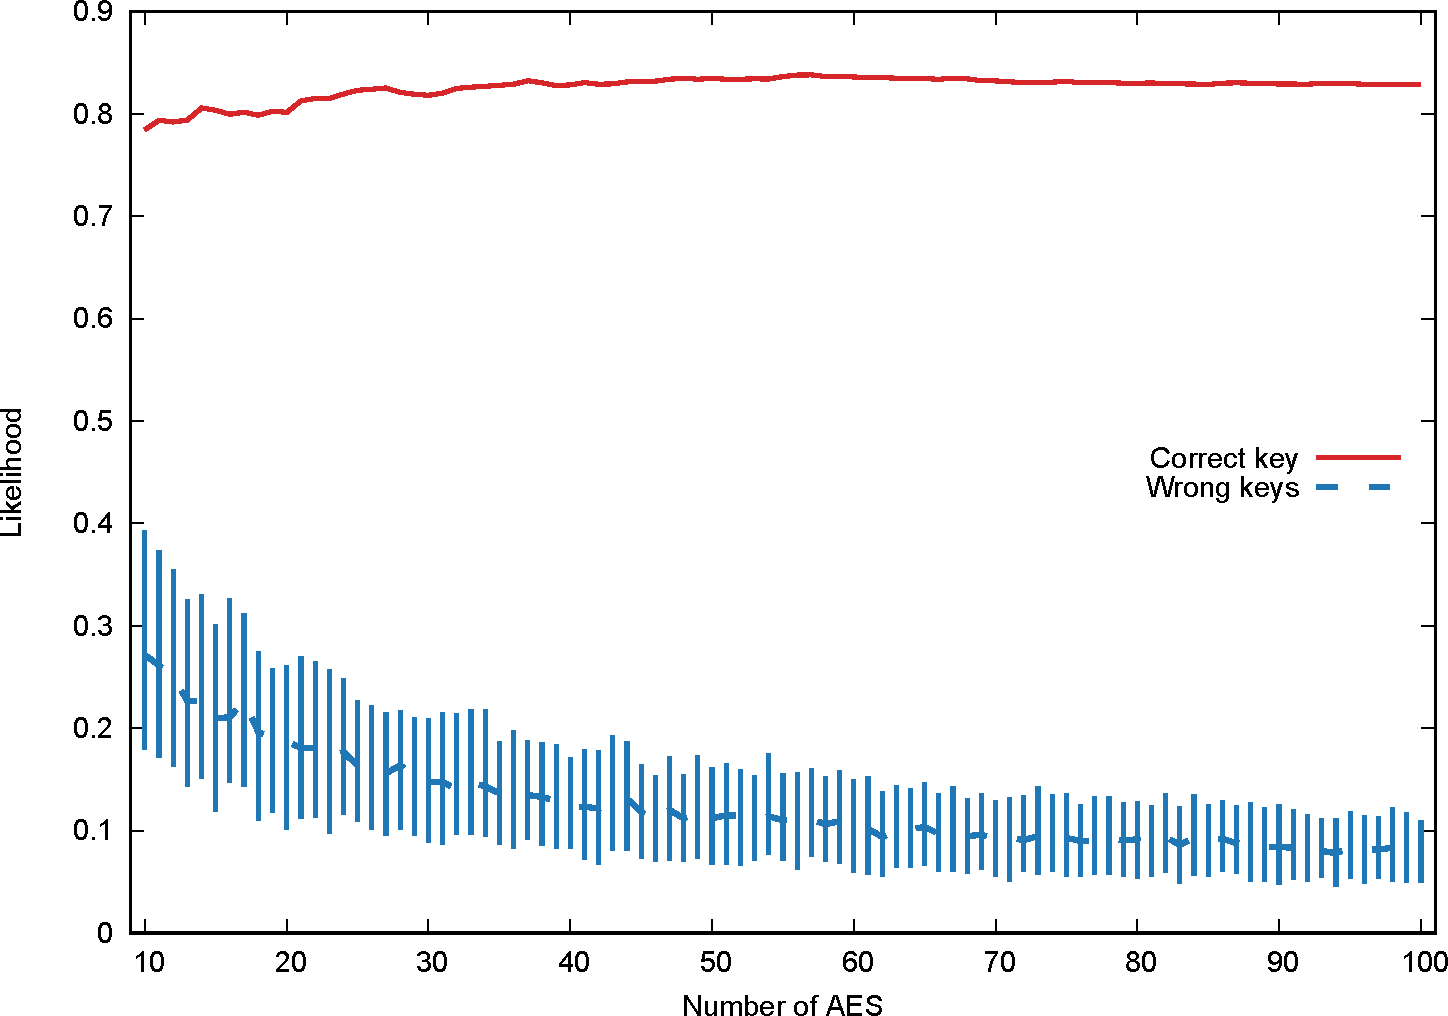
\includegraphics[width=0.5\linewidth]
      {prog_cpa_1r}\label{sfig:oneRound_incN}}
      \subfloat[][Three rounds]{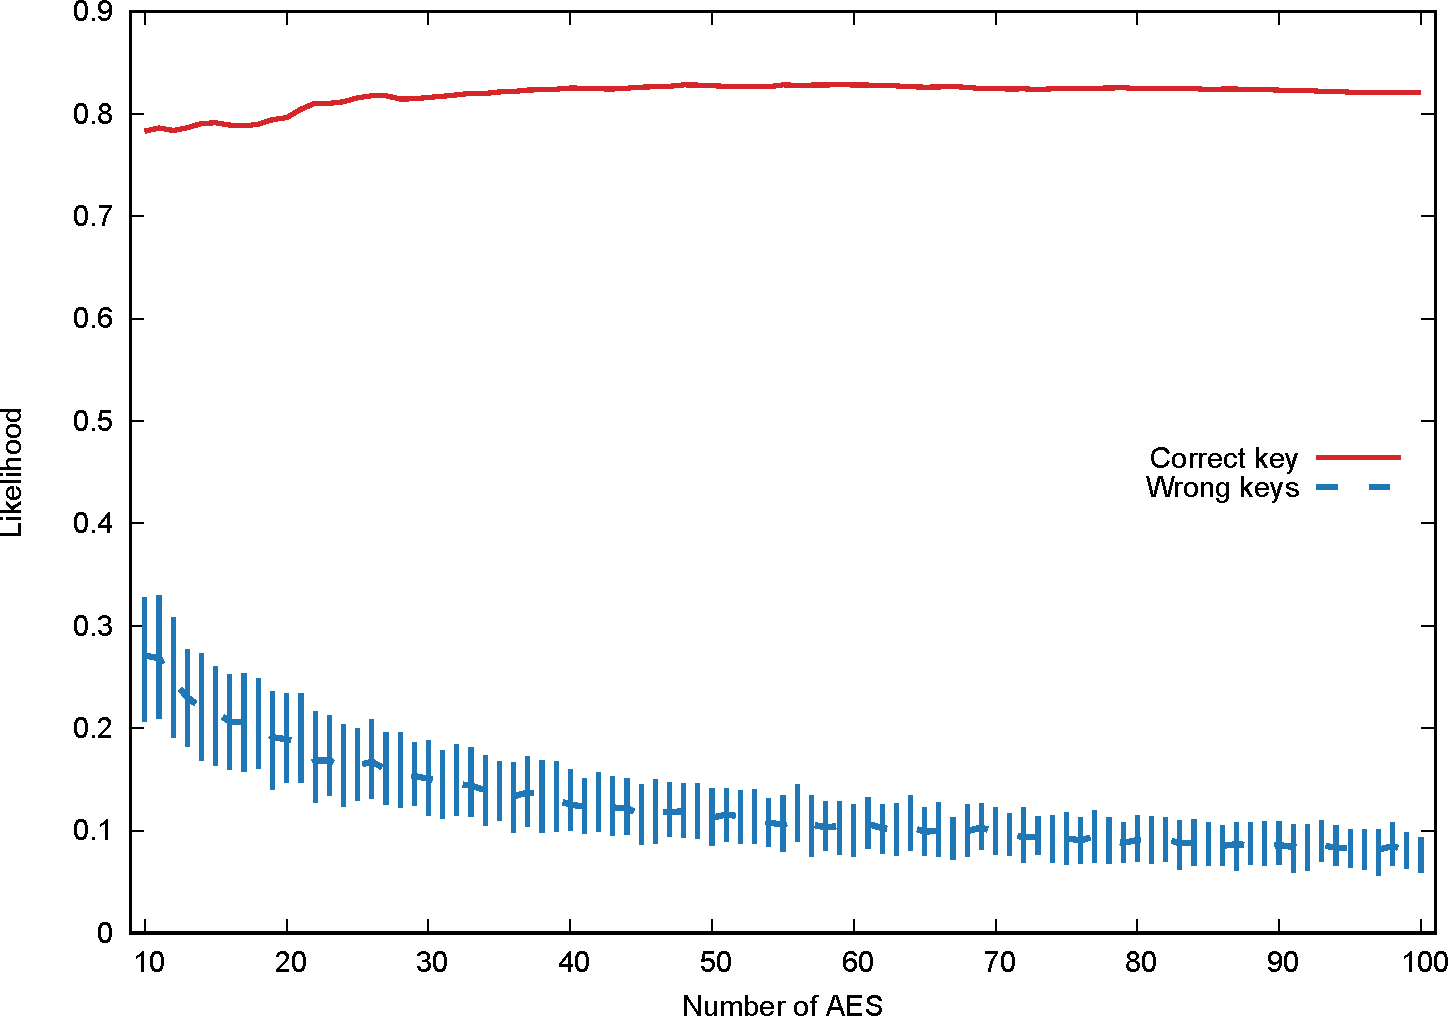
\includegraphics[width=0.5\linewidth]
      {prog_cpa_3r}\label{sfig:threeRounds_incN}}
\caption{Evolution of the likelihood according to an increasing number of AES executions.}\label{fig:likely_grow}
\end{figure}

\subsubsection{Assessment of our Proposal in a Noisy Environment.}
It is well-known that the ChipWhisperer-Lite is mostly noise-free\footnote{According to our measurements, it follows a Gaussian distribution with a standard deviation of $\approx 0.004$.}. To demonstrate the efficiency of our proposal in a noisy environment, the same acquired trace was reused to artificially increase the noise level (\emph{i.e.} by adding a white Gaussian noise).
We plotted in Fig.~\ref{fig:FRRwh} the evolution of the acceptance rate according to an increasing noise standard deviation and a fixed number of executed AES ($N=20$).

As expected, the acceptance rate decreases when the noise standard deviation increases. Moreover, for a fixed noise standard deviation, the more internal states, the higher the acceptance rate.
Finally, we repeated the same experiments when increasing the number of executed AES and  used the Signal-to-Noise Ratio (SNR) rather than the noise standard deviation to better quantify the amount of white noise which is added. The obtained results are depicted in Fig.~\ref{fig:fixed_noised}.

\begin{figure}[ht!]
\centering
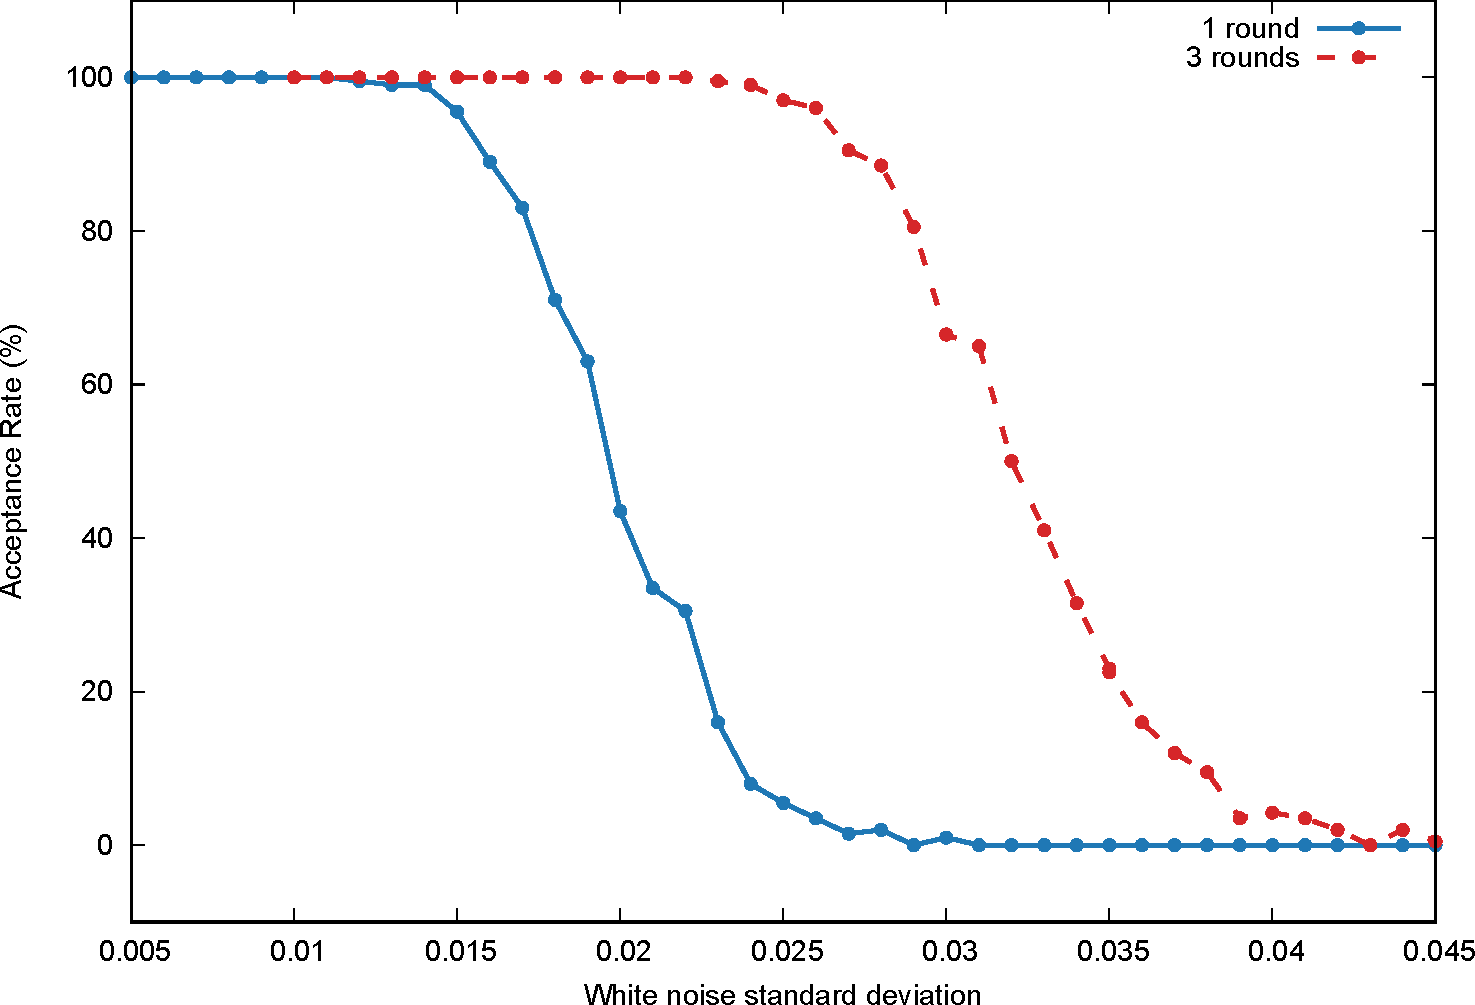
\includegraphics[width=0.9\linewidth]{prob.pdf}
\caption{Evolution of the acceptance rate according to an increasing noise standard deviation and a fixed number of executed AES.}\label{fig:FRRwh}
\end{figure}

\begin{figure}[ht!]
\centering
      \subfloat[][One round]{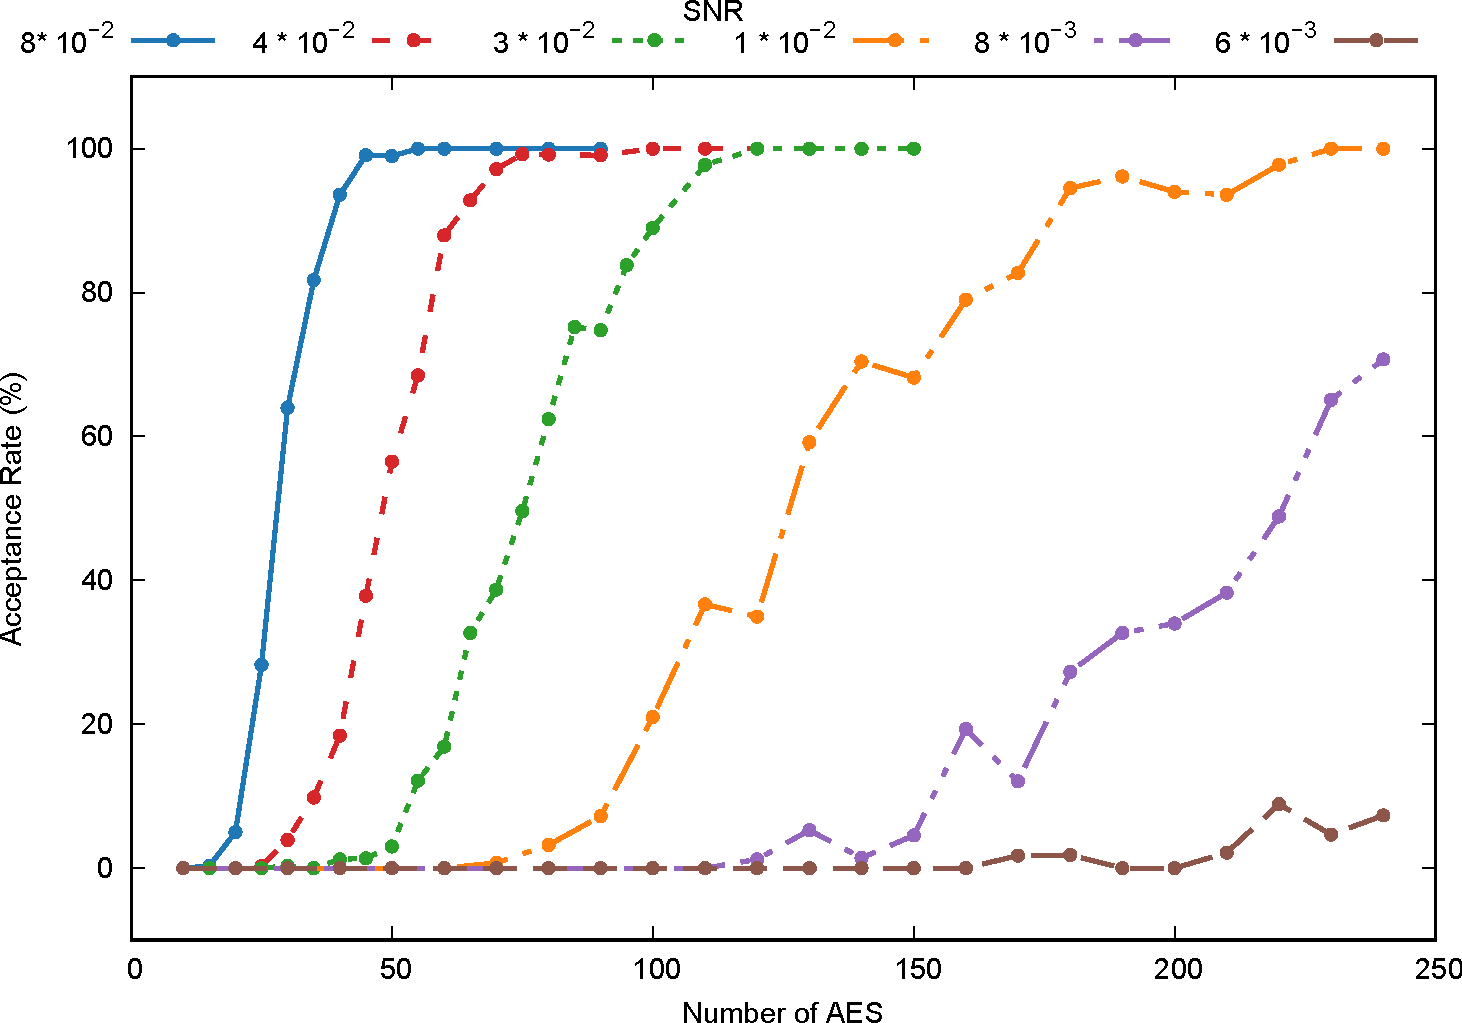
\includegraphics[width=0.5\linewidth]
      {noise_prob_cpa.pdf}\label{sfig:oneRound_incNoise}}
      \subfloat[][Three rounds]{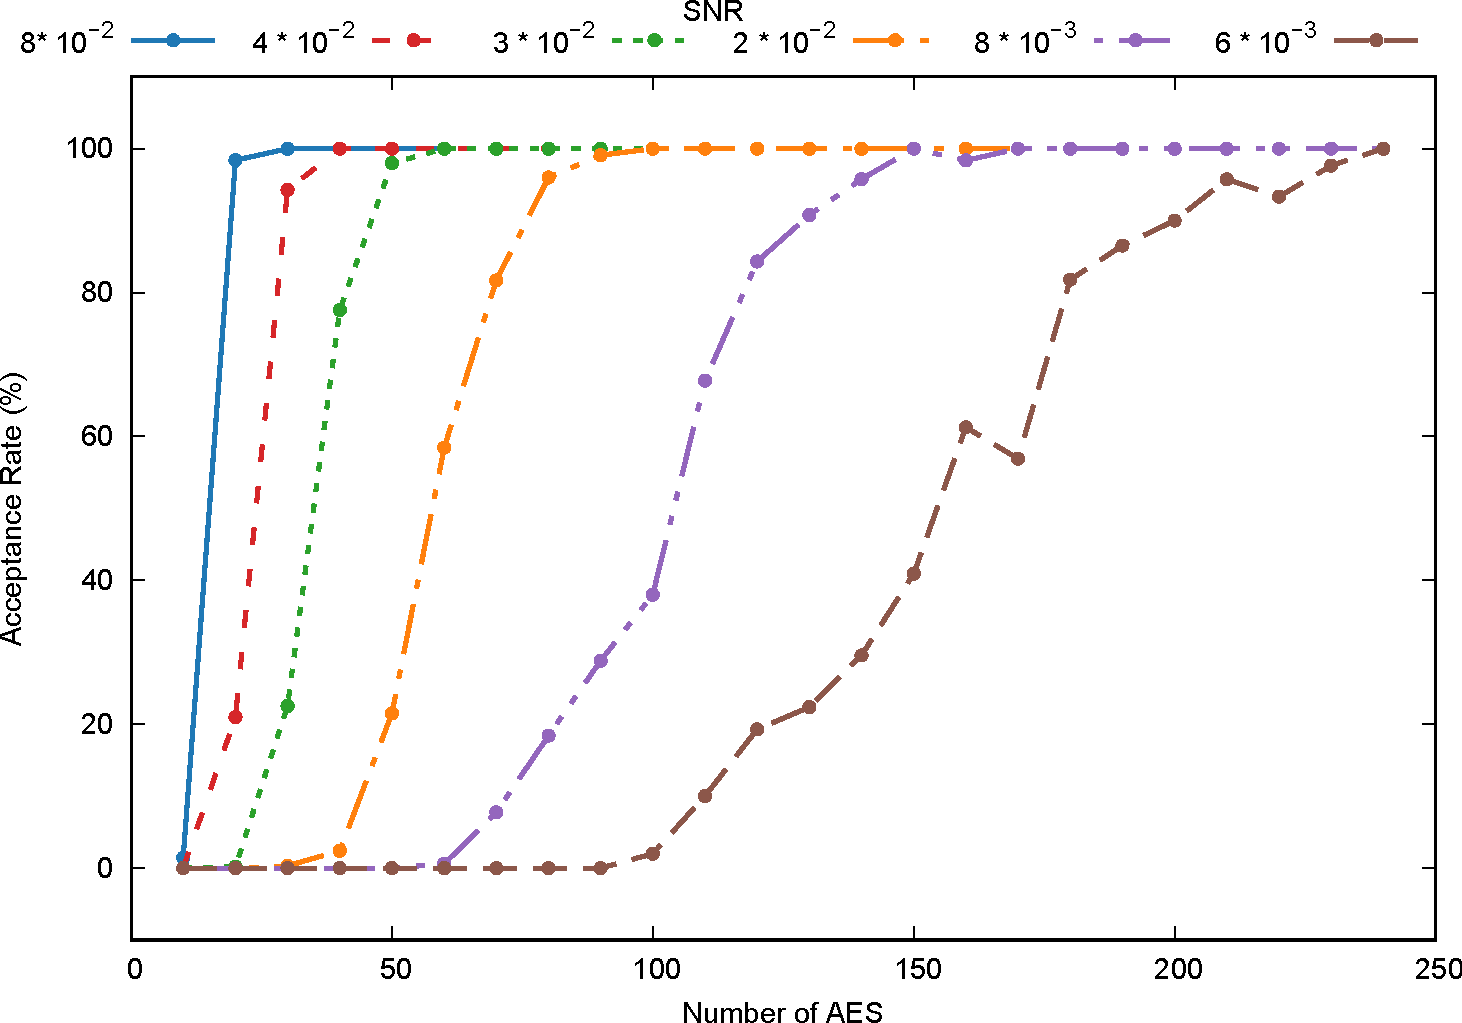
\includegraphics[width=0.5\linewidth]
      {noise_prob_cpa_3r.pdf}\label{sfig:threeRounds_incNoise}}   
\caption{Evolution of the acceptance rate according to an increasing number of executed AES and SNR.}\label{fig:fixed_noised}
\end{figure}
	
From Fig.~\ref{fig:fixed_noised}, one can conclude that in the presence of a significant amount of noise, increasing the number $N$ of AES executions allows the verifier to better distinguish the presence of a genuine prover. Moreover, the number of variables used for the likelihood computation is also of great interest. Indeed, by considering more AES rounds and more internal states per round, the verifier increases the acceptance rate while executing less AES computations.

\add{Regarding the choice of the optimal parameters (\emph{i.e.} number of AES, number of rounds, \dots), it is up to the designer to choose the suitable ones with respect to the the noise level and the required acceptance rate.}


\subsubsection{FAR and FRR Assessment.}\label{ssec:FARFRR}
In this section, we evaluated our proposed authentication protocol with respect to two well-known security metrics: the  \textit{False Acceptance Rate} (FAR) and the \textit{False Rejection Rate} (FRR).
The FAR is the measure of probability that an authentication protocol accepts an unauthorized prover while the FRR is the measure of probability that an authentication protocol rejects a genuine prover.

To do so, we considered in the following an authentication between a verifier and a malicious prover.
We acquired one trace on the ChipWhisperer board corresponding to $N$ executions of leaky AES using wrong session keys at the prover side. We stress the fact that the noise level is similar to the experiments reported in Fig.\ref{sfig:threeRounds_incN} (\emph{i.e.} $\sigma \approx 0.004$). Then, we plotted in Fig.~\ref{fig:proxTest} the evolution of the likelihood $\mathcal{L}_0$ (the red curve) and the estimated mean and mean deviation $(\mu_{\not={0}}, w_{\not={0}})$ of $\Lambda_{\not={0}}$ (the blue dotted curve and bars) according to an increasing number of executed AES when considering three rounds per AES execution.

\begin{figure}[ht!]
\centering
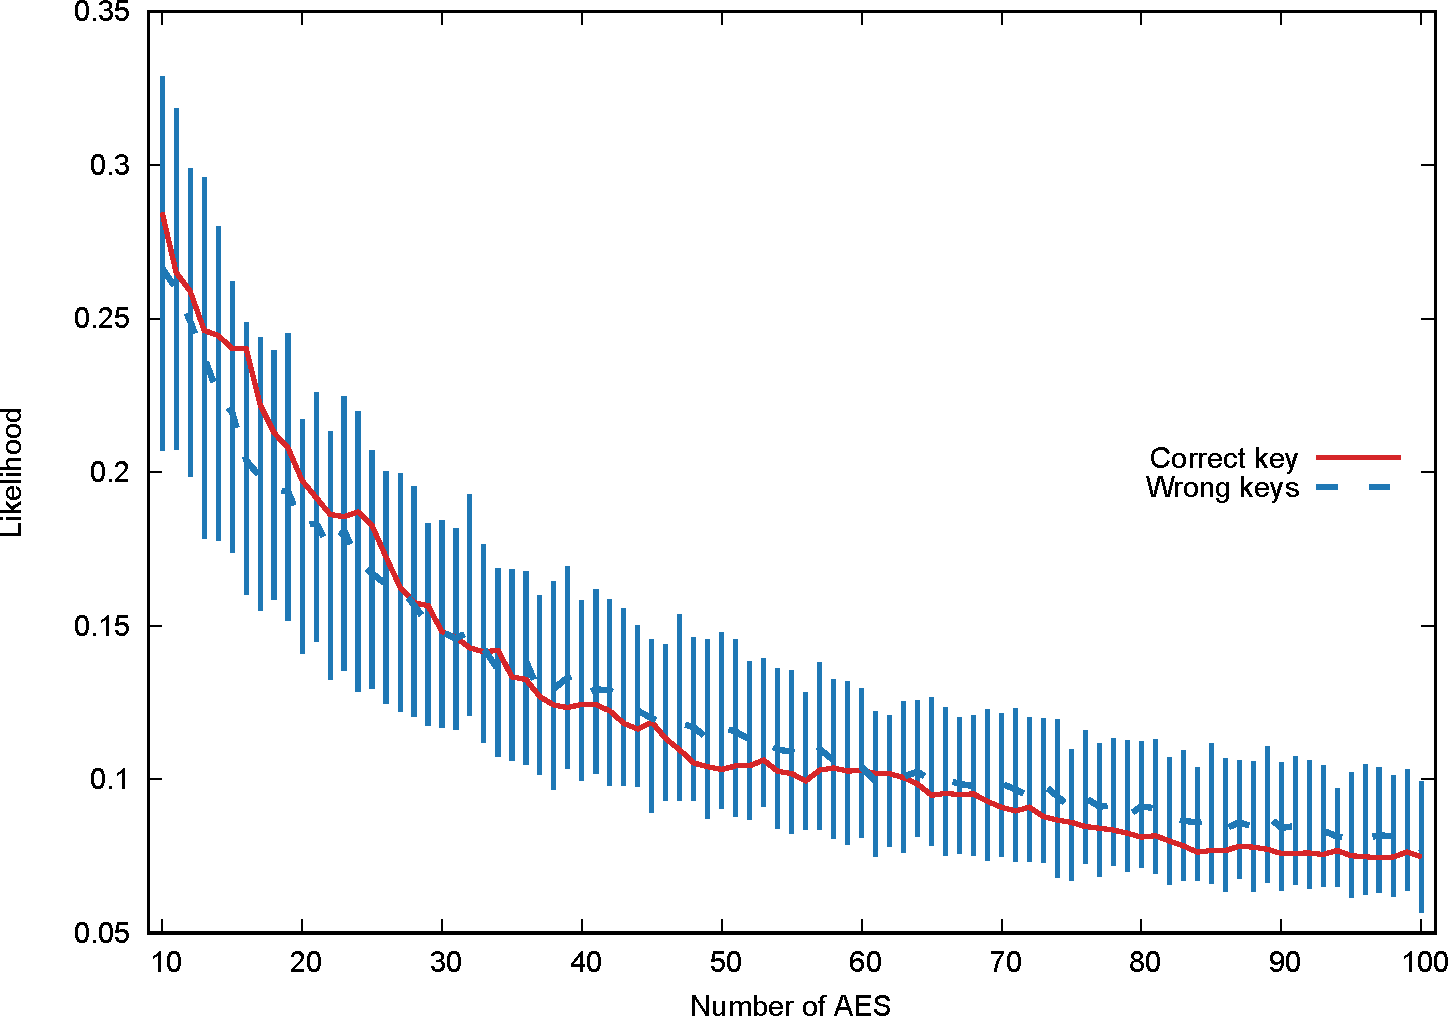
\includegraphics[width=0.7\linewidth]{prog_cpa_3r_false.pdf}
\caption{Evolution of the likelihood according to an increasing number of AES executions when considering a malicious prover.}
\label{fig:proxTest}
\end{figure}

From Fig.~\ref{fig:proxTest}, one can see that the curves overlap and hence the verifier concludes that the prover is a malicious one and rejects the authentication.
So, the obtained results confirm that the FAR of our proposed authentication protocol is almost zero independently of the number of executed AES. We recall that, by design, the theoretical FAR is $2^{-128}$ which the probability that a malicious prover guesses correctly the $128$-bit shared master key $K$. 

Regarding the FRR, we demonstrated in Fig.~\ref{fig:fixed_noised} that in the presence of a genuine prover the acceptance rate decreases (\emph{i.e.} the FRR increases) when the noise standard deviation increases. On the other hand, when the number of executed AES increases and/or when considering several intermediate values then the acceptance rate increases too. This implies that, depending on the application, one can adjust the FRR by tuning the number of executed AES and the number of targeted intermediate values with respect to the noise level. This can be done as a beforehand agreement between the genuine prover and the verifier.

\section{Conclusion}\label{sec:conc}
This work highlights the bright side of side-channel leakage. The traditional doctrine has always exhibited this leakage as a serious practical threat to cryptographic embedded systems. In this paper, we have introduced a new authentication protocol that constructively exploits the side-channel leakage to prevent relay attacks. To be authenticated, the prover performs some cryptographic operations using a beforehand shared master key (either loaded during the personalization phase of the prover or more simply by using the classical Diffie-Hellman key exchange protocol). The verifier eavesdrops the resulting physical leakage and computes the likelihood using the corresponding theoretical predictions. 
When the resulting likelihood is quite high (with respect to the considered proximity criterion) then the prover could be accepted after a last step of validation by exchanging some ciphertexts.
We have argued and confirmed with experiments, that our proposal is secure against both side-channel attacks and relay attacks. Moreover, it solves some security and design issues pinpointed in a previous study~\cite{SakiyamaMMKHMMN15}. Besides, through our experimental validation, we have demonstrated the efficiency of our proposal in terms of FAR and FRR.
       
In view of these promising results, a natural open problem is to validate our proposal in an even more realistic scenario by exploiting for example the electromagnetic leakage captured on a modern smart-card chip.

\bibliographystyle{plain}
\bibliography{physical_authent}

\end{document}
